\section{Analyse de bien-être}

This chapter asks how well a market serves those who trade on it: the question of
\textbf{bien-être} (\textit{welfare}). Its yardstick is the surplus. On the buyers'
side the disponibilité à payer gives the surplus du consommateur; on the sellers'
side the cost gives the surplus du producteur; together they make the surplus total,
which the équilibre de marché maximises.\\

The second half asks what makes an allocation efficient. The answer is the
efficacité de Pareto, drawn first in the boîte d'Edgeworth, where two consumers
share two goods, then against a frontière des possibilités de production, where the
question is what to produce. The two théorèmes du bien-être tie it to the équilibre
concurrentiel. Their assumptions, the critiques of the critère de Pareto, Amartya
Sen's among them, and the approach of John Rawls close the chapter.

\subsection{Disponibilité à payer et surplus}

The buyers' side comes first, with two definitions.

\begin{definition}[Disponibilité à payer (\textit{willingness to pay})]
  \textbf{Disponibilité à payer} = prix maximum que l'on est prêt à payer.
\end{definition}

\begin{definition}[Surplus du consommateur (\textit{consumer surplus})]
  \textbf{Surplus du consommateur} = disponibilité à payer moins le prix payé.
\end{definition}

\begin{example}[Le premier album d'Elvis Presley]
  Four possible buyers want Elvis Presley's first album, each with their own
  disponibilité à payer:
  \begin{center}
    \begin{tabular}{@{}lc@{}}
      \toprule
      Acheteur & Disponibilité à payer \\
      \midrule
      John & 100~\$ \\
      Paul & 80 \\
      George & 70 \\
      Ringo & 50 \\
      \bottomrule
    \end{tabular}
  \end{center}
  The example runs through the rest of this subsection.
\end{example}

\subsubsection{Demande et disponibilité à payer}

The four disponibilités à payer make up the barème de demande for the album. At each
price, the table lists the buyers who buy and the quantité demandée, their number:
\begin{center}
  \begin{tabular}{@{}llc@{}}
    \toprule
    Prix & Acheteurs & Quantité demandée \\
    \midrule
    Plus de 100~\$ & Aucun & 0 \\
    De 80 à 100~\$ & John & 1 \\
    De 70 à 80~\$ & John, Paul & 2 \\
    De 50 à 70~\$ & John, Paul, George & 3 \\
    50~\$ ou moins & John, Paul, George, Ringo & 4 \\
    \bottomrule
  \end{tabular}
\end{center}
The courbe de demande that graphs this barème is a staircase, and its height
reflects the buyers' disponibilité à payer: each step stands at the disponibilité à
payer of one buyer.\\

\begin{figure}[h!]
  \centering
  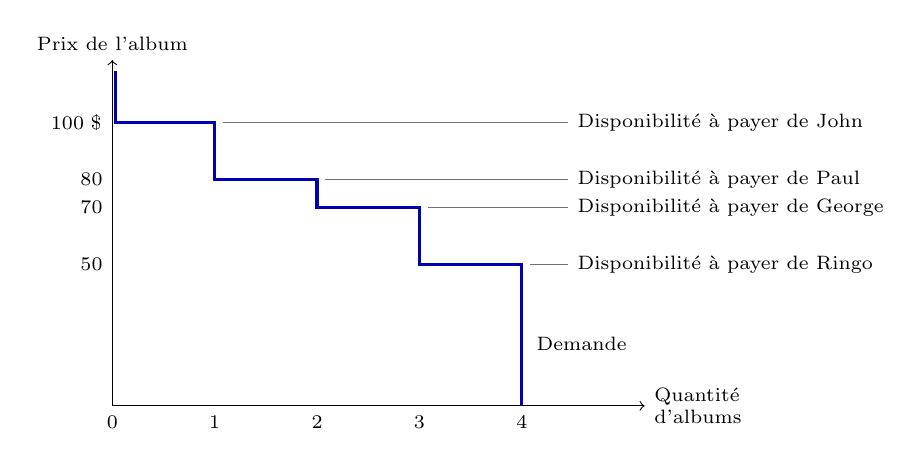
\begin{tikzpicture}[x=1.3cm,y=0.036cm,font=\scriptsize,
      lead/.style={black!55}]
    % axes
    \draw[->] (0,0) -- (5.2,0);
    \draw[->] (0,0) -- (0,122);
    \node[above] at (0,122) {Prix de l'album};
    \node[right,align=left] at (5.2,0) {Quantité\\d'albums};
    \foreach \q in {0,...,4} \node[below] at (\q,0) {$\q$};
    \foreach \p/\l in {50/{$50$},70/{$70$},80/{$80$},100/{$100$~\$}}
      \node[left] at (0,\p) {\l};
    % the step demand curve
    \draw[blue!70!black,very thick] (0.03,118) -- (0.03,100) -- (1,100) -- (1,80)
      -- (2,80) -- (2,70) -- (3,70) -- (3,50) -- (4,50) -- (4,0);
    \node[right] at (4.05,22) {Demande};
    % whose disponibilité à payer each step is
    \foreach \x/\p/\n in {1/100/John, 2/80/Paul, 3/70/George, 4/50/Ringo} {
      \draw[lead] (\x+0.08,\p) -- (4.45,\p);
      \node[right] at (4.45,\p) {Disponibilité à payer de \n};
    }
  \end{tikzpicture}
  \caption*{\small Le barème de demande et la courbe de demande de l'album. The
  courbe de demande is a staircase; its height at each unit is the disponibilité à
  payer of one of the four buyers.}
\end{figure}

On the courbe de demande, the surplus du consommateur is measured as the area below
the curve and above the price. A lower price raises it.

\begin{example}[Le surplus du consommateur à 80~\$ et à 70~\$]
  At a price of 80~\$ only John buys the album, and the surplus du consommateur is
  John's: $100 - 80 = 20$~\$. At 70~\$ John and Paul buy it. John's surplus is
  $100 - 70 = 30$~\$ and Paul's $80 - 70 = 10$~\$, so the surplus du consommateur
  totals 40~\$.
\end{example}

\begin{figure}[h!]
  \centering
  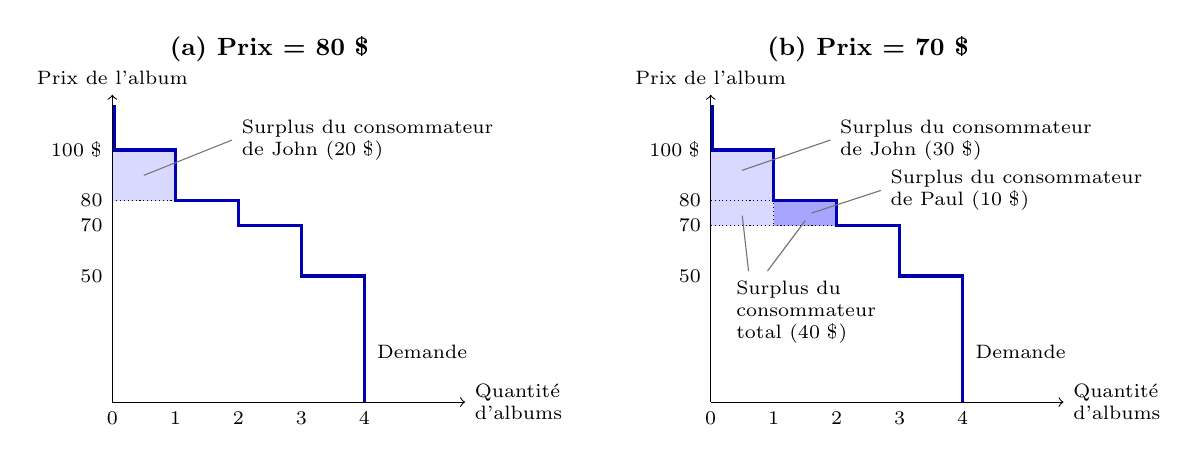
\begin{tikzpicture}[x=0.8cm,y=0.032cm,font=\scriptsize,
      lead/.style={black!55}]
    % ---- panel (a): price 80
    \begin{scope}
      \fill[blue!15] (0,80) rectangle (1,100);
      \draw[densely dotted] (0,80) -- (1,80);
      \draw[->] (0,0) -- (5.6,0);
      \draw[->] (0,0) -- (0,122);
      \node[above] at (0,122) {Prix de l'album};
      \node[right,align=left] at (5.6,0) {Quantité\\d'albums};
      \foreach \q in {0,...,4} \node[below] at (\q,0) {$\q$};
      \foreach \p/\l in {50/{$50$},70/{$70$},80/{$80$},100/{$100$~\$}}
        \node[left] at (0,\p) {\l};
      \draw[blue!70!black,very thick] (0.03,118) -- (0.03,100) -- (1,100) -- (1,80)
        -- (2,80) -- (2,70) -- (3,70) -- (3,50) -- (4,50) -- (4,0);
      \node[right] at (4.05,20) {Demande};
      \node[align=left,anchor=west] (j) at (1.9,104) {Surplus du consommateur\\de John (20~\$)};
      \draw[lead] (j.west) -- (0.5,90);
      \node[font=\small\bfseries] at (2.5,140) {(a) Prix = 80~\$};
    \end{scope}
    % ---- panel (b): price 70
    \begin{scope}[xshift=7.6cm]
      \fill[blue!15] (0,70) rectangle (1,100);
      \fill[blue!35] (1,70) rectangle (2,80);
      \draw[densely dotted] (0,70) -- (2,70);
      \draw[densely dotted] (0,80) -- (1,80) -- (1,70);
      \draw[->] (0,0) -- (5.6,0);
      \draw[->] (0,0) -- (0,122);
      \node[above] at (0,122) {Prix de l'album};
      \node[right,align=left] at (5.6,0) {Quantité\\d'albums};
      \foreach \q in {0,...,4} \node[below] at (\q,0) {$\q$};
      \foreach \p/\l in {50/{$50$},70/{$70$},80/{$80$},100/{$100$~\$}}
        \node[left] at (0,\p) {\l};
      \draw[blue!70!black,very thick] (0.03,118) -- (0.03,100) -- (1,100) -- (1,80)
        -- (2,80) -- (2,70) -- (3,70) -- (3,50) -- (4,50) -- (4,0);
      \node[right] at (4.05,20) {Demande};
      \node[align=left,anchor=west] (j) at (1.9,104) {Surplus du consommateur\\de John (30~\$)};
      \draw[lead] (j.west) -- (0.5,92);
      \node[align=left,anchor=west] (p) at (2.7,84) {Surplus du consommateur\\de Paul (10~\$)};
      \draw[lead] (p.west) -- (1.6,75);
      \node[align=left,anchor=north west] (t) at (0.25,52) {Surplus du\\consommateur\\total (40~\$)};
      \draw[lead] (0.6,52) -- (0.5,74);
      \draw[lead] (0.9,52) -- (1.5,72);
      \node[font=\small\bfseries] at (2.5,140) {(b) Prix = 70~\$};
    \end{scope}
  \end{tikzpicture}
  \caption*{\small Mesurer le surplus du consommateur avec la courbe de demande. At
  80~\$ the surplus du consommateur is 20~\$, John's alone; at 70~\$ it is 40~\$,
  John's 30~\$ and Paul's 10~\$. The shaded area lies below the courbe de demande and
  above the price.}
\end{figure}

\begin{figure}[h!]
  \centering
  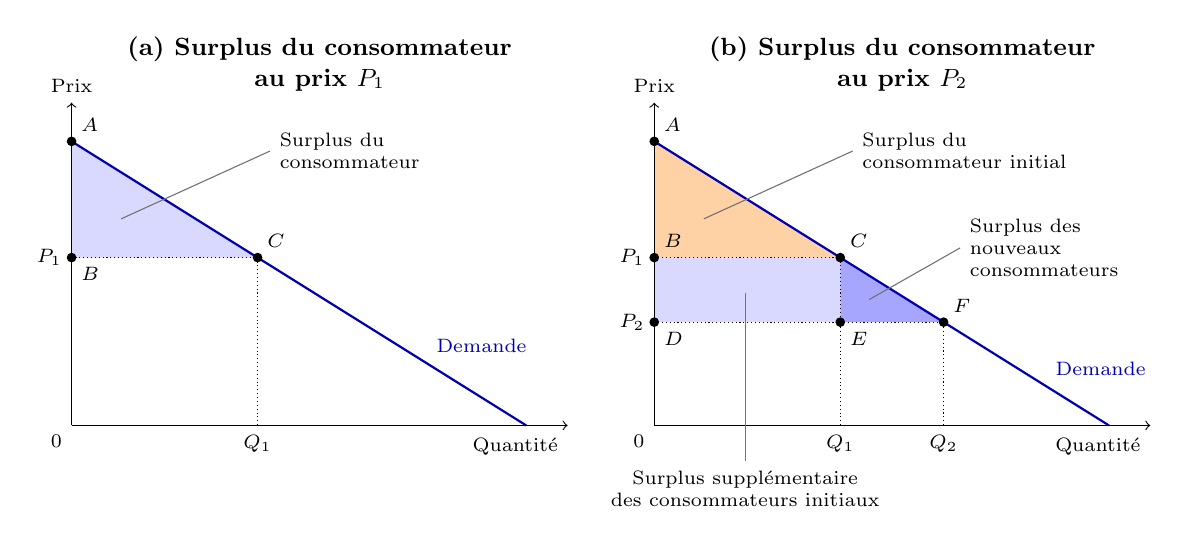
\begin{tikzpicture}[x=1.05cm,y=0.82cm,font=\scriptsize,
      dot/.style={circle,fill=black,inner sep=0pt,minimum size=3.5pt},
      lead/.style={black!55}]
    % ---- panel (a): the first price
    \begin{scope}
      \fill[blue!15] (0,4.4) -- (0,2.6) -- (2.25,2.6) -- cycle;
      \draw[densely dotted] (0,2.6) -- (2.25,2.6) -- (2.25,0);
      \draw[->] (0,0) -- (6,0);
      \draw[->] (0,0) -- (0,5);
      \node[above] at (0,5) {Prix};
      \node[below left] at (6,-0.05) {Quantité};
      \node[below left] at (0,0) {$0$};
      \draw[blue!70!black,thick] (0,4.4) -- (5.5,0) node[pos=0.78,above right] {Demande};
      \node[left] at (0,2.6) {$P_1$};
      \node[below] at (2.25,0) {$Q_1$};
      \foreach \p/\l/\a in {(0,4.4)/A/above right,(0,2.6)/B/below right,(2.25,2.6)/C/above right}
        { \node[dot] at \p {}; \node[\a] at \p {$\l$}; }
      \node[align=left,anchor=west] (s) at (2.4,4.25) {Surplus du\\consommateur};
      \draw[lead] (s.west) -- (0.6,3.2);
      \node[font=\small\bfseries,align=center] at (3,5.6) {(a) Surplus du consommateur\\au prix $P_1$};
    \end{scope}
    % ---- panel (b): the second price
    \begin{scope}[xshift=7.4cm]
      \fill[orange!35] (0,4.4) -- (0,2.6) -- (2.25,2.6) -- cycle;
      \fill[blue!15] (0,2.6) rectangle (2.25,1.6);
      \fill[blue!35] (2.25,2.6) -- (2.25,1.6) -- (3.5,1.6) -- cycle;
      \draw[densely dotted] (0,2.6) -- (2.25,2.6) -- (2.25,0);
      \draw[densely dotted] (0,1.6) -- (3.5,1.6) -- (3.5,0);
      \draw[->] (0,0) -- (6,0);
      \draw[->] (0,0) -- (0,5);
      \node[above] at (0,5) {Prix};
      \node[below left] at (6,-0.05) {Quantité};
      \node[below left] at (0,0) {$0$};
      \draw[blue!70!black,thick] (0,4.4) -- (5.5,0) node[pos=0.86,above right] {Demande};
      \node[left] at (0,2.6) {$P_1$};
      \node[left] at (0,1.6) {$P_2$};
      \node[below] at (2.25,0) {$Q_1$};
      \node[below] at (3.5,0) {$Q_2$};
      \foreach \p/\l/\a in {(0,4.4)/A/above right,(0,2.6)/B/above right,(2.25,2.6)/C/above right,
          (0,1.6)/D/below right,(2.25,1.6)/E/below right,(3.5,1.6)/F/above right}
        { \node[dot] at \p {}; \node[\a] at \p {$\l$}; }
      \node[align=left,anchor=west] (i) at (2.4,4.25) {Surplus du\\consommateur initial};
      \draw[lead] (i.west) -- (0.6,3.2);
      \node[align=left,anchor=west] (n) at (3.7,2.75) {Surplus des\\nouveaux\\consommateurs};
      \draw[lead] (n.west) -- (2.6,1.95);
      \node[align=center,anchor=north] (o) at (1.1,-0.55) {Surplus supplémentaire\\des consommateurs initiaux};
      \draw[lead] (o.north) -- (1.1,2.05);
      \node[font=\small\bfseries,align=center] at (3,5.6) {(b) Surplus du consommateur\\au prix $P_2$};
    \end{scope}
  \end{tikzpicture}
  \caption*{\small L'effet du prix sur le surplus du consommateur. At $P_1$ the
  surplus du consommateur is the triangle $ABC$; at the lower $P_2$ it is the
  triangle $ADF$, the initial surplus $ABC$ plus $BCED$ for the consumers already in
  the market and $CEF$ for the new ones.}
\end{figure}

The same reading holds for a linear courbe de demande (figure «~L'effet du prix sur
le surplus du consommateur~»). At the price $P_1$ the quantité demandée is $Q_1$, and
the surplus du consommateur is the area of the triangle $ABC$. When the price falls
from $P_1$ to $P_2$, the quantité demandée rises from $Q_1$ to $Q_2$, and the
surplus du consommateur rises to the area of the triangle $ADF$. The increase, the
area $BCFD$, has two parts:
\begin{itemize}
  \item the area $BCED$, because the consumers already in the market now pay less;
  \item the area $CEF$, because new consumers enter the market at the lower price.
\end{itemize}

\subsection{Surplus du producteur}

The sellers' side mirrors the buyers'. Where a buyer has a highest price they will
pay, a seller has a lowest price they will accept, and the gap between price and that
cost is their surplus.

\begin{definition}[Disponibilité à vendre (\textit{willingness to sell})]
  La \textbf{disponibilité à vendre} est le prix minimum auquel le vendeur accepte
  de vendre, c'est-à-dire son coût.
\end{definition}

\begin{definition}[Surplus du producteur (\textit{producer surplus})]
  Le \textbf{surplus du producteur} est le prix de vente moins le coût.
\end{definition}

\begin{remark}[Formulation du cours]
  «~Disponibilité à vendre = différence entre le prix de vente et le coût.~»
\end{remark}

\begin{example}[Repeindre la maison]
  Four possible sellers offer to repaint a house, each at their own cost:
  \begin{center}
    \begin{tabular}{@{}lc@{}}
      \toprule
      Vendeur & Coût \\
      \midrule
      Mary & 900~\$ \\
      Frida & 800 \\
      Georgia & 600 \\
      Grandma & 500 \\
      \bottomrule
    \end{tabular}
  \end{center}
  The example runs through the rest of this subsection.
\end{example}

The four costs make up the barème d'offre. At each price, the table lists the
sellers who sell and the quantité offerte, their number:
\begin{center}
  \begin{tabular}{@{}llc@{}}
    \toprule
    Prix & Vendeurs & Quantité offerte \\
    \midrule
    900~\$ ou plus & Mary, Frida, Georgia, Grandma & 4 \\
    De 800 à 900~\$ & Frida, Georgia, Grandma & 3 \\
    De 600 à 800~\$ & Georgia, Grandma & 2 \\
    De 500 à 600~\$ & Grandma & 1 \\
    Moins de 500~\$ & Aucun & 0 \\
    \bottomrule
  \end{tabular}
\end{center}
The courbe d'offre that graphs this barème is again a staircase, and its height
reflects the sellers' costs: each step stands at the cost of one seller.\\

\begin{figure}[h!]
  \centering
  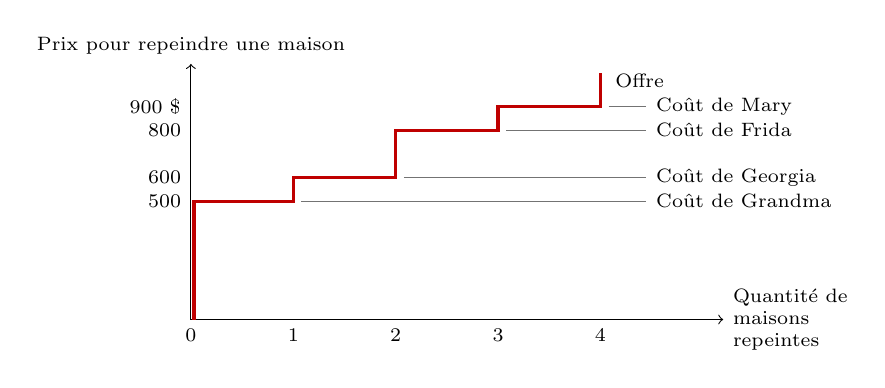
\begin{tikzpicture}[x=1.3cm,y=0.0030cm,font=\scriptsize,
      lead/.style={black!55}]
    % axes
    \draw[->] (0,0) -- (5.2,0);
    \draw[->] (0,0) -- (0,1080);
    \node[above] at (0,1080) {Prix pour repeindre une maison};
    \node[right,align=left] at (5.2,0) {Quantité de\\maisons\\repeintes};
    \foreach \q in {0,...,4} \node[below] at (\q,0) {$\q$};
    \foreach \p/\l in {500/{$500$},600/{$600$},800/{$800$},900/{$900$~\$}}
      \node[left] at (0,\p) {\l};
    % the step supply curve
    \draw[red!75!black,very thick] (0.03,0) -- (0.03,500) -- (1,500) -- (1,600)
      -- (2,600) -- (2,800) -- (3,800) -- (3,900) -- (4,900) -- (4,1040);
    \node[right] at (4.05,1010) {Offre};
    % whose cost each step is
    \foreach \x/\p/\n in {1/500/Grandma, 2/600/Georgia, 3/800/Frida, 4/900/Mary} {
      \draw[lead] (\x+0.08,\p) -- (4.45,\p);
      \node[right] at (4.45,\p) {Coût de \n};
    }
  \end{tikzpicture}
  \caption*{\small Le barème d'offre et la courbe d'offre. The courbe d'offre is a
  staircase; its height at each unit is the cost of one of the four sellers.}
\end{figure}

On the courbe d'offre, the surplus du producteur is measured as the area above the
curve and below the price. A higher price raises it.

\begin{example}[Le surplus du producteur à 600~\$ et à 800~\$]
  At a price of 600~\$ only Grandma sells, and the surplus du producteur is Grandma's:
  $600 - 500 = 100$~\$. At 800~\$ Grandma and Georgia sell. Grandma's surplus is
  $800 - 500 = 300$~\$ and Georgia's $800 - 600 = 200$~\$, so the surplus du
  producteur totals 500~\$.
\end{example}

\begin{figure}[h!]
  \centering
  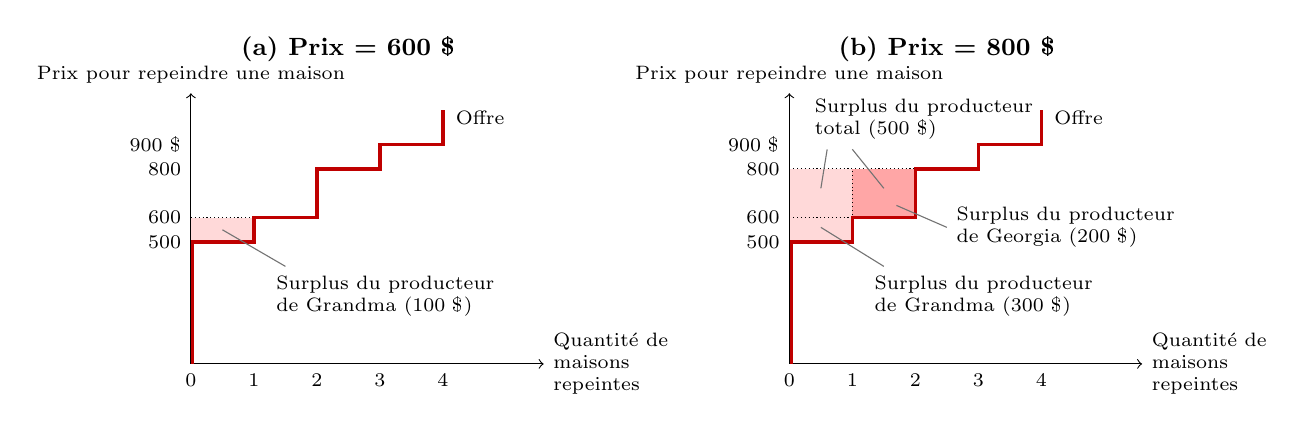
\begin{tikzpicture}[x=0.8cm,y=0.0031cm,font=\scriptsize,
      lead/.style={black!55}]
    % ---- panel (a): price 600
    \begin{scope}
      \fill[red!15] (0,500) rectangle (1,600);
      \draw[densely dotted] (0,600) -- (1,600);
      \draw[->] (0,0) -- (5.6,0);
      \draw[->] (0,0) -- (0,1110);
      \node[above] at (0,1110) {Prix pour repeindre une maison};
      \node[right,align=left] at (5.6,0) {Quantité de\\maisons\\repeintes};
      \foreach \q in {0,...,4} \node[below] at (\q,0) {$\q$};
      \foreach \p/\l in {500/{$500$},600/{$600$},800/{$800$},900/{$900$~\$}}
        \node[left] at (0,\p) {\l};
      \draw[red!75!black,very thick] (0.03,0) -- (0.03,500) -- (1,500) -- (1,600)
        -- (2,600) -- (2,800) -- (3,800) -- (3,900) -- (4,900) -- (4,1040);
      \node[right] at (4.05,1010) {Offre};
      \node[align=left,anchor=north west] (g) at (1.2,400) {Surplus du producteur\\de Grandma (100~\$)};
      \draw[lead] (1.5,400) -- (0.5,550);
      \node[font=\small\bfseries] at (2.5,1290) {(a) Prix = 600~\$};
    \end{scope}
    % ---- panel (b): price 800
    \begin{scope}[xshift=7.6cm]
      \fill[red!15] (0,500) rectangle (1,800);
      \fill[red!35] (1,600) rectangle (2,800);
      \draw[densely dotted] (0,800) -- (2,800);
      \draw[densely dotted] (0,600) -- (1,600) -- (1,800);
      \draw[->] (0,0) -- (5.6,0);
      \draw[->] (0,0) -- (0,1110);
      \node[above] at (0,1110) {Prix pour repeindre une maison};
      \node[right,align=left] at (5.6,0) {Quantité de\\maisons\\repeintes};
      \foreach \q in {0,...,4} \node[below] at (\q,0) {$\q$};
      \foreach \p/\l in {500/{$500$},600/{$600$},800/{$800$},900/{$900$~\$}}
        \node[left] at (0,\p) {\l};
      \draw[red!75!black,very thick] (0.03,0) -- (0.03,500) -- (1,500) -- (1,600)
        -- (2,600) -- (2,800) -- (3,800) -- (3,900) -- (4,900) -- (4,1040);
      \node[right] at (4.05,1010) {Offre};
      \node[align=left,anchor=south west] (t) at (0.25,880) {Surplus du producteur\\total (500~\$)};
      \draw[lead] (0.6,880) -- (0.5,720);
      \draw[lead] (1.0,880) -- (1.5,720);
      \node[align=left,anchor=west] (gg) at (2.5,560) {Surplus du producteur\\de Georgia (200~\$)};
      \draw[lead] (gg.west) -- (1.7,650);
      \node[align=left,anchor=north west] (gm) at (1.2,400) {Surplus du producteur\\de Grandma (300~\$)};
      \draw[lead] (1.5,400) -- (0.5,560);
      \node[font=\small\bfseries] at (2.5,1290) {(b) Prix = 800~\$};
    \end{scope}
  \end{tikzpicture}
  \caption*{\small Mesurer le surplus du producteur avec la courbe d'offre. At
  600~\$ the surplus du producteur is 100~\$, Grandma's alone; at 800~\$ it is
  500~\$, Grandma's 300~\$ and Georgia's 200~\$. The shaded area lies above the
  courbe d'offre and below the price.}
\end{figure}

\begin{figure}[h!]
  \centering
  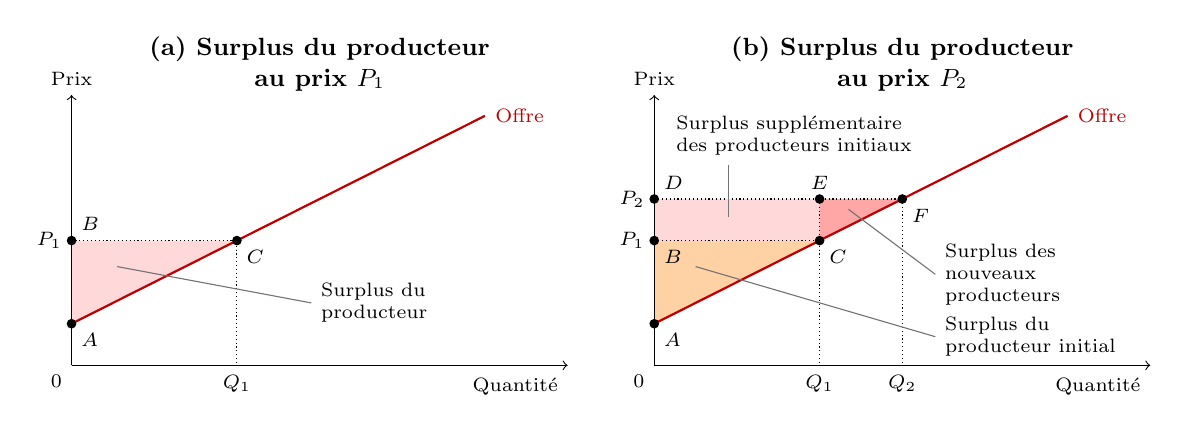
\begin{tikzpicture}[x=1.05cm,y=0.66cm,font=\scriptsize,
      dot/.style={circle,fill=black,inner sep=0pt,minimum size=3.5pt},
      lead/.style={black!55}]
    % ---- panel (a): the first price
    \begin{scope}
      \fill[red!15] (0,0.8) -- (0,2.4) -- (2,2.4) -- cycle;
      \draw[densely dotted] (0,2.4) -- (2,2.4) -- (2,0);
      \draw[->] (0,0) -- (6,0);
      \draw[->] (0,0) -- (0,5.2);
      \node[above] at (0,5.2) {Prix};
      \node[below left] at (6,-0.05) {Quantité};
      \node[below left] at (0,0) {$0$};
      \draw[red!75!black,thick] (0,0.8) -- (5,4.8) node[right] {Offre};
      \node[left] at (0,2.4) {$P_1$};
      \node[below] at (2,0) {$Q_1$};
      \foreach \p/\l/\a in {(0,0.8)/A/below right,(0,2.4)/B/above right,(2,2.4)/C/below right}
        { \node[dot] at \p {}; \node[\a] at \p {$\l$}; }
      \node[align=left,anchor=west] (s) at (2.9,1.2) {Surplus du\\producteur};
      \draw[lead] (s.west) -- (0.55,1.9);
      \node[font=\small\bfseries,align=center] at (3,5.8) {(a) Surplus du producteur\\au prix $P_1$};
    \end{scope}
    % ---- panel (b): the second price
    \begin{scope}[xshift=7.4cm]
      \fill[orange!35] (0,0.8) -- (0,2.4) -- (2,2.4) -- cycle;
      \fill[red!15] (0,2.4) rectangle (2,3.2);
      \fill[red!35] (2,2.4) -- (2,3.2) -- (3,3.2) -- cycle;
      \draw[densely dotted] (0,2.4) -- (2,2.4) -- (2,0);
      \draw[densely dotted] (0,3.2) -- (3,3.2) -- (3,0);
      \draw[densely dotted] (2,3.2) -- (2,2.4);
      \draw[->] (0,0) -- (6,0);
      \draw[->] (0,0) -- (0,5.2);
      \node[above] at (0,5.2) {Prix};
      \node[below left] at (6,-0.05) {Quantité};
      \node[below left] at (0,0) {$0$};
      \draw[red!75!black,thick] (0,0.8) -- (5,4.8) node[right] {Offre};
      \node[left] at (0,2.4) {$P_1$};
      \node[left] at (0,3.2) {$P_2$};
      \node[below] at (2,0) {$Q_1$};
      \node[below] at (3,0) {$Q_2$};
      \foreach \p/\l/\a in {(0,0.8)/A/below right,(0,2.4)/B/below right,(2,2.4)/C/below right,
          (0,3.2)/D/above right,(2,3.2)/E/above,(3,3.2)/F/below right}
        { \node[dot] at \p {}; \node[\a] at \p {$\l$}; }
      \node[align=left,anchor=south west] (o) at (0.15,3.85) {Surplus supplémentaire\\des producteurs initiaux};
      \draw[lead] (0.9,3.85) -- (0.9,2.85);
      \node[align=left,anchor=west] (n) at (3.4,1.75) {Surplus des\\nouveaux\\producteurs};
      \draw[lead] (n.west) -- (2.35,3.0);
      \node[align=left,anchor=west] (i) at (3.4,0.55) {Surplus du\\producteur initial};
      \draw[lead] (i.west) -- (0.5,1.9);
      \node[font=\small\bfseries,align=center] at (3,5.8) {(b) Surplus du producteur\\au prix $P_2$};
    \end{scope}
  \end{tikzpicture}
  \caption*{\small L'effet du prix sur le surplus du producteur. At $P_1$ the
  surplus du producteur is the triangle $ABC$; at the higher $P_2$ it is the
  triangle $ADF$, the initial surplus $ABC$ plus $BCED$ for the producers already in
  the market and $CEF$ for the new ones.}
\end{figure}

The same reading holds for a linear courbe d'offre (figure «~L'effet du prix sur le
surplus du producteur~»). At the price $P_1$ the quantité offerte is $Q_1$, and the
surplus du producteur is the area of the triangle $ABC$. When the price rises from
$P_1$ to $P_2$, the quantité offerte rises from $Q_1$ to $Q_2$, and the surplus du
producteur rises to the area of the triangle $ADF$. The increase, the area $BCFD$,
has two parts:
\begin{itemize}
  \item the area $BCED$, because the producers already in the market now receive
    more;
  \item the area $CEF$, because new producers enter the market at the higher price.
\end{itemize}

\subsection{Surplus total}

Buyers and sellers meet at the équilibre de marché. The \textbf{surplus total}
(\textit{total surplus}) is the sum of the surplus du consommateur and the surplus du
producteur. At the équilibre it is the area between the courbe d'offre and the
courbe de demande up to the quantité d'équilibre: the surplus du consommateur lies
above the prix d'équilibre, the surplus du producteur below it.\\

\begin{figure}[h!]
  \centering
  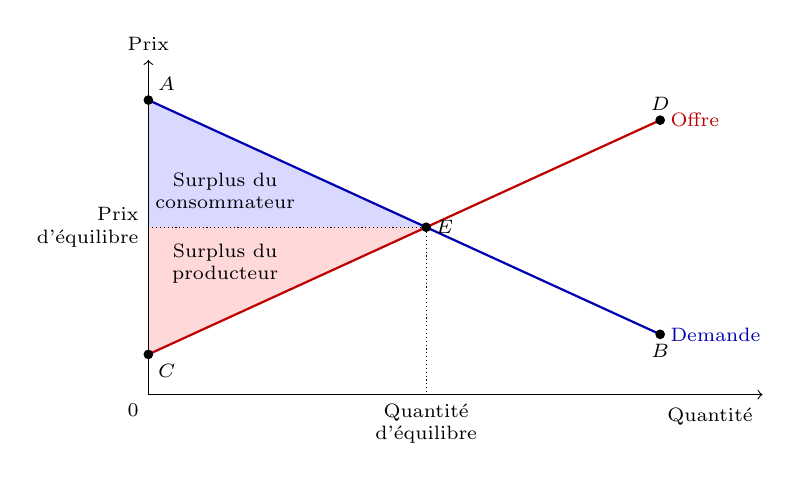
\begin{tikzpicture}[x=1.3cm,y=0.85cm,font=\scriptsize,
      dot/.style={circle,fill=black,inner sep=0pt,minimum size=3.5pt}]
    \fill[blue!15] (0,4.4) -- (2.714,2.5) -- (0,2.5) -- cycle;
    \fill[red!15] (0,2.5) -- (2.714,2.5) -- (0,0.6) -- cycle;
    \draw[densely dotted] (0,2.5) -- (2.714,2.5) -- (2.714,0);
    \draw[->] (0,0) -- (6,0);
    \draw[->] (0,0) -- (0,5);
    \node[above] at (0,5) {Prix};
    \node[below left] at (6,-0.05) {Quantité};
    \node[below left] at (0,0) {$0$};
    \draw[blue!70!black,thick] (0,4.4) -- (5,0.9) node[right] {Demande};
    \draw[red!75!black,thick] (0,0.6) -- (5,4.1) node[right] {Offre};
    \node[left,align=right] at (0,2.5) {Prix\\d'équilibre};
    \node[below,align=center] at (2.714,0) {Quantité\\d'équilibre};
    \node[align=center] at (0.75,3.05) {Surplus du\\consommateur};
    \node[align=center] at (0.75,1.95) {Surplus du\\producteur};
    \foreach \p/\l/\a in {(0,4.4)/A/above right,(5,0.9)/B/below,(0,0.6)/C/below right,
        (5,4.1)/D/above,(2.714,2.5)/E/right}
      { \node[dot] at \p {}; \node[\a] at \p {$\l$}; }
  \end{tikzpicture}
  \caption*{\small Le surplus du consommateur et le surplus du producteur à
  l'équilibre de marché. Their sum, the surplus total, is the area between the
  courbe d'offre and the courbe de demande up to the quantité d'équilibre.}
\end{figure}

\begin{figure}[h!]
  \centering
  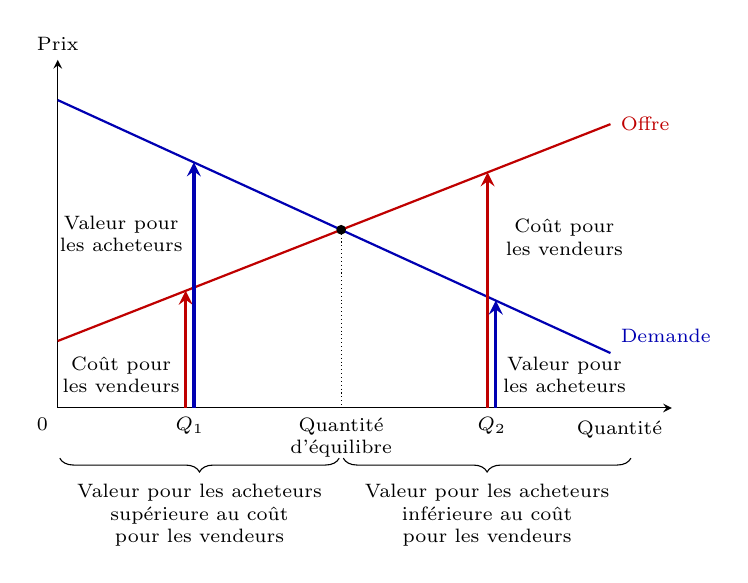
\begin{tikzpicture}[x=1.3cm,y=0.85cm,font=\scriptsize,>=stealth,
      dot/.style={circle,fill=black,inner sep=0pt,minimum size=3.5pt},
      brc/.style={decorate,decoration={brace,amplitude=5pt,mirror}}]
    \draw[->] (0,0) -- (6,0);
    \draw[->] (0,0) -- (0,5.2);
    \node[above] at (0,5.2) {Prix};
    \node[below left] at (6,-0.05) {Quantité};
    \node[below left] at (0,0) {$0$};
    \draw[blue!70!black,thick] (0,4.6) -- (5.4,0.82) node[above right] {Demande};
    \draw[red!75!black,thick] (0,1.0) -- (5.4,4.24) node[right] {Offre};
    \draw[densely dotted] (2.769,2.662) -- (2.769,0);
    \node[dot] at (2.769,2.662) {};
    % at Q1 < equilibrium quantity
    \draw[->,red!75!black,very thick] (1.25,0) -- (1.25,1.75);
    \draw[->,blue!70!black,very thick] (1.33,0) -- (1.33,3.669);
    \node[align=center] at (0.62,2.6) {Valeur pour\\les acheteurs};
    \node[align=center] at (0.62,0.5) {Coût pour\\les vendeurs};
    % at Q2 > equilibrium quantity
    \draw[->,red!75!black,very thick] (4.2,0) -- (4.2,3.52);
    \draw[->,blue!70!black,very thick] (4.28,0) -- (4.28,1.604);
    \node[align=center] at (4.95,2.55) {Coût pour\\les vendeurs};
    \node[align=center] at (4.95,0.5) {Valeur pour\\les acheteurs};
    % quantities
    \node[below] at (1.29,0) {$Q_1$};
    \node[below,align=center] at (2.769,0) {Quantité\\d'équilibre};
    \node[below] at (4.24,0) {$Q_2$};
    \draw[brc] (0.02,-0.75) -- (2.75,-0.75)
      node[midway,below=6pt,align=center,text width=3.3cm]
      {Valeur pour les acheteurs supérieure au coût pour les vendeurs};
    \draw[brc] (2.79,-0.75) -- (5.6,-0.75)
      node[midway,below=6pt,align=center,text width=3.3cm]
      {Valeur pour les acheteurs inférieure au coût pour les vendeurs};
  \end{tikzpicture}
  \caption*{\small L'efficacité de la quantité d'équilibre. Below the quantité
  d'équilibre the value to the buyers exceeds the cost to the sellers; above it the
  cost exceeds the value. The équilibre de marché maximises the surplus total.}
\end{figure}

The équilibre de marché maximises the surplus total. The heights of the two curves
show why. At a quantity below the quantité d'équilibre, such as $Q_1$, the value of
the good to the buyers, read on the courbe de demande, exceeds its cost to the
sellers, read on the courbe d'offre. At a quantity above it, such as $Q_2$, the cost
to the sellers exceeds the value to the buyers. Therefore the équilibre de marché
maximises the sum of the surplus du producteur and the surplus du consommateur.

\subsection{L'efficacité de Pareto}

The surplus measures what one market creates. The second criterion asks of a whole
allocation whether anyone could be made better off without making someone else
worse off.

\begin{definition}[Efficacité de Pareto (\textit{Pareto efficiency})]
  L'\textbf{efficacité de Pareto}~: situation dans laquelle on ne peut pas
  améliorer la situation de quelqu'un sans détériorer la situation de quelqu'un
  d'autre.
\end{definition}

The tool for studying it is the \textbf{boîte d'Edgeworth} (\textit{Edgeworth
box}), built for two goods and two consumers.

\subsubsection{Boîte d'Edgeworth}

\begin{figure}[h!]
  \centering
  \begin{tikzpicture}[x=1cm,y=1cm,font=\scriptsize,>=stealth,
      dot/.style={circle,fill=black,inner sep=0pt,minimum size=3.5pt},
      lab/.style={fill=white,inner sep=0.8pt,outer sep=2.5pt,text=black}]
    \draw (0,0) rectangle (6,4.5);
    \draw[dashed] (2.2,0) -- (2.2,4.5);
    \draw[dashed] (0,1.8) -- (6,1.8);
    \node[dot] at (2.2,1.8) {};
    \node[above right,lab] at (2.2,1.8) {$Q$};
    % origins and the direction in which each consumer's quantities grow
    \node[below left] at (0,0) {$O_A$};
    \node[above right] at (6,4.5) {$O_B$};
    \draw[->] (0.35,-0.3) -- (1.5,-0.3);
    \draw[->] (-0.3,0.35) -- (-0.3,1.3);
    \draw[->] (5.65,4.8) -- (4.5,4.8);
    \draw[->] (6.3,4.15) -- (6.3,3.2);
    % ends of the quantities measured from O_A
    \node[below] at (2.2,0) {$X$};
    \node[below] at (6,0) {$X$};
    \node[left] at (0,1.8) {$Y$};
    \node[left] at (0,4.5) {$Y$};
    \node[above] at (2.2,4.5) {$X$};
    \node[right] at (6,1.8) {$Y$};
    \node[below] at (3,-0.55) {Bien $X$};
    \node[rotate=90] at (-0.85,2.25) {Bien $Y$};
  \end{tikzpicture}
  \caption*{\small La boîte d'Edgeworth. $A$'s quantities are measured from $O_A$,
  rightward and upward; $B$'s from $O_B$, leftward and downward. The point $Q$ is one
  allocation: the dashed lines split each good between $A$ (the part next to $O_A$)
  and $B$ (the part next to $O_B$).}
\end{figure}

\begin{figure}[h!]
  \centering
  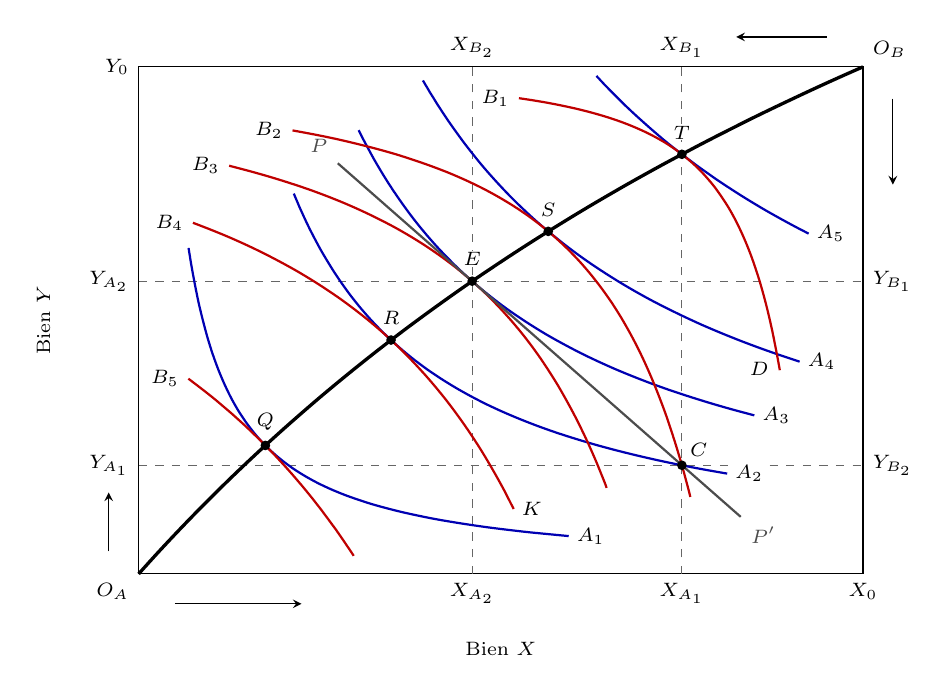
\begin{tikzpicture}[x=1.15cm,y=1.15cm,font=\scriptsize,>=stealth,
      dot/.style={circle,fill=black,inner sep=0pt,minimum size=3.5pt},
      acurve/.style={blue!70!black,thick},
      bcurve/.style={red!75!black,thick},
      ccurve/.style={black,very thick},
      pline/.style={black!70,thick},
      lab/.style={fill=white,inner sep=0.5pt,outer sep=2.5pt,text=black}]
    % the box
    \draw (0,0) rectangle (8,5.6);
    \node[below left] at (0,0) {$O_A$};
    \node[above right] at (8,5.6) {$O_B$};
    \node[below] at (8,0) {$X_0$};
    \node[left] at (0,5.6) {$Y_0$};
    \draw[->] (0.4,-0.33) -- (1.8,-0.33);
    \draw[->] (-0.33,0.25) -- (-0.33,0.9);
    \draw[->] (7.6,5.93) -- (6.6,5.93);
    \draw[->] (8.33,5.25) -- (8.33,4.3);
    \node[below] at (4,-0.65) {Bien $X$};
    \node[rotate=90] at (-1.05,2.8) {Bien $Y$};
    % quantities held at E and at C
    \draw[dashed,black!60] (3.684,0) -- (3.684,5.6);
    \draw[dashed,black!60] (6,0) -- (6,5.6);
    \draw[dashed,black!60] (0,3.233) -- (8,3.233);
    \draw[dashed,black!60] (0,1.2) -- (8,1.2);
    \node[below] at (3.684,0) {$X_{A_2}$};
    \node[below] at (6,0) {$X_{A_1}$};
    \node[above] at (3.684,5.6) {$X_{B_2}$};
    \node[above] at (6,5.6) {$X_{B_1}$};
    \node[left] at (0,3.233) {$Y_{A_2}$};
    \node[left] at (0,1.2) {$Y_{A_1}$};
    \node[right] at (8,3.233) {$Y_{B_1}$};
    \node[right] at (8,1.2) {$Y_{B_2}$};
    % A's courbes d'indifférence A_1 ... A_5 (lower-right labels)
    \draw[acurve] plot[smooth] coordinates {(0.552,3.600) (0.555,3.579) (0.565,3.517) (0.581,3.419) (0.604,3.291) (0.633,3.139) (0.668,2.972) (0.711,2.796) (0.759,2.617) (0.814,2.440) (0.876,2.268) (0.944,2.105) (1.018,1.951) (1.099,1.807) (1.187,1.674) (1.281,1.551) (1.381,1.438) (1.488,1.335) (1.601,1.241) (1.721,1.154) (1.848,1.075) (1.980,1.003) (2.120,0.937) (2.265,0.877) (2.418,0.822) (2.576,0.771) (2.742,0.725) (2.913,0.682) (3.091,0.643) (3.276,0.606) (3.467,0.573) (3.665,0.542) (3.869,0.513) (4.079,0.487) (4.296,0.462) (4.520,0.440) (4.750,0.418)}
      node[right,lab] {$A_{1}$};
    \draw[acurve] plot[smooth] coordinates {(1.714,4.200) (1.718,4.191) (1.729,4.164) (1.748,4.120) (1.773,4.060) (1.807,3.985) (1.847,3.898) (1.895,3.799) (1.951,3.691) (2.013,3.576) (2.084,3.456) (2.161,3.332) (2.246,3.206) (2.338,3.079) (2.438,2.953) (2.545,2.829) (2.660,2.707) (2.781,2.589) (2.911,2.474) (3.047,2.363) (3.191,2.256) (3.343,2.154) (3.502,2.056) (3.668,1.963) (3.841,1.874) (4.022,1.790) (4.211,1.710) (4.406,1.634) (4.609,1.562) (4.820,1.494) (5.038,1.429) (5.263,1.368) (5.496,1.310) (5.736,1.255) (5.983,1.203) (6.238,1.154) (6.500,1.108)}
      node[right,lab] {$A_{2}$};
    \draw[acurve] plot[smooth] coordinates {(2.430,4.900) (2.434,4.893) (2.444,4.873) (2.461,4.840) (2.484,4.794) (2.515,4.736) (2.552,4.667) (2.595,4.588) (2.646,4.500) (2.703,4.405) (2.767,4.303) (2.838,4.196) (2.916,4.084) (3.000,3.969) (3.091,3.852) (3.189,3.734) (3.293,3.616) (3.405,3.498) (3.523,3.380) (3.647,3.265) (3.779,3.151) (3.917,3.040) (4.062,2.931) (4.214,2.826) (4.372,2.724) (4.538,2.624) (4.710,2.529) (4.888,2.436) (5.074,2.347) (5.266,2.261) (5.465,2.179) (5.670,2.100) (5.883,2.024) (6.102,1.952) (6.328,1.882) (6.561,1.815) (6.800,1.751)}
      node[right,lab] {$A_{3}$};
    \draw[acurve] plot[smooth] coordinates {(3.140,5.450) (3.143,5.444) (3.153,5.428) (3.169,5.400) (3.192,5.362) (3.220,5.314) (3.256,5.257) (3.297,5.190) (3.346,5.115) (3.400,5.033) (3.461,4.945) (3.529,4.850) (3.602,4.751) (3.683,4.647) (3.769,4.540) (3.862,4.431) (3.962,4.320) (4.068,4.207) (4.180,4.094) (4.299,3.981) (4.424,3.868) (4.556,3.757) (4.694,3.646) (4.838,3.537) (4.989,3.430) (5.146,3.326) (5.310,3.223) (5.480,3.123) (5.657,3.025) (5.840,2.931) (6.029,2.839) (6.225,2.749) (6.427,2.663) (6.636,2.579) (6.851,2.498) (7.072,2.420) (7.300,2.344)}
      node[right,lab] {$A_{4}$};
    \draw[acurve] plot[smooth] coordinates {(5.056,5.500) (5.058,5.498) (5.063,5.492) (5.072,5.482) (5.085,5.469) (5.101,5.451) (5.121,5.430) (5.144,5.405) (5.172,5.377) (5.202,5.345) (5.237,5.310) (5.275,5.272) (5.316,5.231) (5.361,5.186) (5.410,5.140) (5.463,5.090) (5.519,5.039) (5.579,4.985) (5.642,4.929) (5.709,4.871) (5.779,4.811) (5.853,4.750) (5.931,4.688) (6.013,4.625) (6.098,4.560) (6.186,4.495) (6.279,4.429) (6.374,4.362) (6.474,4.295) (6.577,4.228) (6.684,4.160) (6.794,4.093) (6.908,4.025) (7.026,3.958) (7.147,3.891) (7.272,3.824) (7.400,3.758)}
      node[right,lab] {$A_{5}$};
    % B's courbes d'indifférence B_1 ... B_5 (upper-left labels)
    \draw[bcurve] plot[smooth] coordinates {(4.200,5.254) (4.358,5.230) (4.511,5.204) (4.660,5.175) (4.805,5.144) (4.945,5.110) (5.080,5.073) (5.211,5.033) (5.338,4.989) (5.460,4.941) (5.578,4.889) (5.692,4.832) (5.801,4.771) (5.905,4.704) (6.005,4.631) (6.101,4.551) (6.192,4.466) (6.278,4.373) (6.361,4.273) (6.438,4.165) (6.512,4.051) (6.581,3.928) (6.645,3.799) (6.705,3.664) (6.761,3.523) (6.812,3.378) (6.859,3.231) (6.901,3.084) (6.939,2.939) (6.972,2.800) (7.001,2.669) (7.025,2.550) (7.045,2.447) (7.061,2.363) (7.072,2.301) (7.079,2.263) (7.081,2.250)};
    \node[left] at (4.200,5.254) {$B_{1}$};
    \draw[bcurve] plot[smooth] coordinates {(1.700,4.898) (1.941,4.853) (2.175,4.805) (2.402,4.752) (2.622,4.696) (2.836,4.636) (3.042,4.570) (3.242,4.500) (3.436,4.425) (3.622,4.344) (3.802,4.257) (3.975,4.163) (4.141,4.063) (4.300,3.956) (4.453,3.841) (4.598,3.719) (4.737,3.589) (4.870,3.451) (4.995,3.306) (5.114,3.153) (5.226,2.994) (5.331,2.828) (5.429,2.656) (5.521,2.480) (5.605,2.302) (5.683,2.122) (5.754,1.944) (5.819,1.770) (5.876,1.602) (5.927,1.444) (5.971,1.299) (6.009,1.169) (6.039,1.058) (6.063,0.969) (6.080,0.904) (6.090,0.863) (6.093,0.850)};
    \node[left] at (1.700,4.898) {$B_{2}$};
    \draw[bcurve] plot[smooth] coordinates {(1.000,4.508) (1.228,4.448) (1.450,4.385) (1.666,4.318) (1.875,4.248) (2.078,4.173) (2.274,4.094) (2.464,4.010) (2.647,3.922) (2.824,3.830) (2.995,3.732) (3.159,3.630) (3.316,3.523) (3.468,3.411) (3.612,3.294) (3.751,3.173) (3.883,3.047) (4.008,2.917) (4.127,2.784) (4.240,2.648) (4.346,2.510) (4.446,2.370) (4.539,2.229) (4.626,2.090) (4.706,1.951) (4.780,1.816) (4.848,1.686) (4.909,1.561) (4.964,1.444) (5.012,1.336) (5.054,1.239) (5.089,1.154) (5.118,1.082) (5.141,1.025) (5.157,0.984) (5.166,0.958) (5.169,0.950)};
    \node[left] at (1.000,4.508) {$B_{3}$};
    \draw[bcurve] plot[smooth] coordinates {(0.600,3.878) (0.804,3.799) (1.003,3.717) (1.195,3.631) (1.382,3.541) (1.563,3.447) (1.739,3.350) (1.908,3.249) (2.072,3.144) (2.230,3.036) (2.383,2.923) (2.529,2.808) (2.670,2.689) (2.805,2.567) (2.935,2.442) (3.058,2.314) (3.176,2.185) (3.288,2.054) (3.395,1.922) (3.495,1.790) (3.590,1.658) (3.679,1.527) (3.763,1.398) (3.840,1.272) (3.912,1.149) (3.978,1.032) (4.039,0.920) (4.093,0.814) (4.142,0.717)};
    \node[left] at (0.600,3.878) {$B_{4}$};
    \draw[bcurve] plot[smooth] coordinates {(0.550,2.156) (0.650,2.080) (0.747,2.005) (0.842,1.929) (0.933,1.852) (1.022,1.776) (1.108,1.699) (1.191,1.623) (1.271,1.546) (1.349,1.471) (1.423,1.395) (1.495,1.321) (1.564,1.247) (1.630,1.175) (1.694,1.103) (1.754,1.033) (1.812,0.965) (1.867,0.898) (1.919,0.834) (1.968,0.771) (2.015,0.711) (2.058,0.653) (2.099,0.598) (2.137,0.546) (2.173,0.498) (2.205,0.452) (2.234,0.410) (2.261,0.371) (2.285,0.336) (2.306,0.304) (2.325,0.277) (2.340,0.254) (2.353,0.234) (2.363,0.219) (2.370,0.209) (2.374,0.202) (2.375,0.200)};
    \node[left] at (0.550,2.156) {$B_{5}$};
    % courbe de contrats
    \draw[ccurve] plot[smooth] coordinates {(0.000,0.000) (0.200,0.221) (0.400,0.435) (0.600,0.643) (0.800,0.845) (1.000,1.042) (1.200,1.233) (1.400,1.419) (1.600,1.600) (1.800,1.776) (2.000,1.948) (2.200,2.115) (2.400,2.278) (2.600,2.437) (2.800,2.592) (3.000,2.743) (3.200,2.890) (3.400,3.034) (3.600,3.175) (3.800,3.312) (4.000,3.446) (4.200,3.577) (4.400,3.705) (4.600,3.830) (4.800,3.953) (5.000,4.073) (5.200,4.190) (5.400,4.305) (5.600,4.417) (5.800,4.527) (6.000,4.634) (6.200,4.740) (6.400,4.843) (6.600,4.944) (6.800,5.044) (7.000,5.141) (7.200,5.236) (7.400,5.330) (7.600,5.422) (7.800,5.512) (8.000,5.600)};
    % the straight line PP' through E and C
    \draw[pline] (2.200,4.535) node[above left] {$P$} -- (6.650,0.630) node[below right] {$P'$};
    % points
    \node[dot] at (1.400,1.419) {}; \node[above=2.5pt,lab] at (1.400,1.419) {$Q$};
    \node[dot] at (2.788,2.583) {}; \node[above=2.5pt,lab] at (2.788,2.583) {$R$};
    \node[dot] at (3.684,3.233) {}; \node[above=2.5pt,lab] at (3.684,3.233) {$E$};
    \node[dot] at (4.524,3.783) {}; \node[above=2.5pt,lab] at (4.524,3.783) {$S$};
    \node[dot] at (6.000,4.634) {}; \node[above=2.5pt,lab] at (6.000,4.634) {$T$};
    \node[dot] at (6.000,1.200) {}; \node[above right,lab] at (6.000,1.200) {$C$};
    \node[below left,lab] at (7.049,2.428) {$D$};
    \node[right,lab] at (4.142,0.717) {$K$};
  \end{tikzpicture}
  \caption*{\small L'équilibre général de l'échange dans la boîte d'Edgeworth. $X_0$ and
  $Y_0$ are the total quantities of the two goods. $A_1$ to $A_5$ are $A$'s courbes
  d'indifférence, $A$'s utilité rising towards the NE; $B_1$ to $B_5$ are $B$'s, $B$'s
  utilité rising towards the SO. The thick curve from $O_A$ to $O_B$, the courbe de
  contrats, passes through the points where a courbe of $A$ touches a courbe of $B$:
  $Q$ ($A_1$ and $B_5$), $R$ ($A_2$ and $B_4$), $E$ ($A_3$ and $B_3$), $S$ ($A_4$
  and $B_2$) and $T$ ($A_5$ and $B_1$). At $C$, $A_2$ and $B_2$ cross without
  touching: there $A$ holds $X_{A_1}$ and $Y_{A_1}$, and $B$ holds $X_{B_1}$ and
  $Y_{B_2}$. At $E$, $A$ holds $X_{A_2}$ and $Y_{A_2}$, and $B$ holds $X_{B_2}$ and
  $Y_{B_1}$. $D$ is where $A_4$ crosses $B_1$, and $K$ a labelled
  point at the lower end of $B_4$, beside $A_1$. The straight line $PP'$ passes
  through $C$ and touches $A_3$ and $B_3$ at $E$.}
\end{figure}

The two consumers are $A$ and $B$, the two goods $X$ and $Y$. The width of the box
is the total quantity of bien $X$, its height the total quantity of bien $Y$. $A$'s
quantities are measured from the origin $O_A$, at the bottom-left corner, $B$'s from
the origin $O_B$, at the top-right corner, so each point of the box, such as $Q$ in
the figure «~La boîte d'Edgeworth~», divides both goods between the two consumers.
Moving across the box (NE = nord-est, SO = sud-ouest) makes one better off and the
other worse off:
\begin{itemize}
  \item l'utilité de $A$ augmente vers le NE, l'utilité de $B$ diminue~;
  \item l'utilité de $B$ augmente vers le SO, l'utilité de $A$ diminue.
\end{itemize}

Each consumer's courbes d'indifférence can be drawn in the box, $A$'s from $O_A$ and
$B$'s from $O_B$. Where one of $A$'s courbes meets one of $B$'s, an équilibre asks
for more than a crossing:

\begin{prop}
  La condition d'équilibre impose que les deux courbes d'indifférence soient
  tangentes.
\end{prop}

\begin{example}[Partir du point $C$]
  «~Si la situation de départ est le point $C$, que se passe-t-il~? Vers le point
  $R$~? vers le point $S$~? vers le point $E$~?~» --- «~En partant de $C$, tous les
  points sur la courbe entre $R$ et $S$ sont des situations d'équilibre
  potentielles.~»\\

  The curve is the one through the points of tangency. As drawn, $R$ lies on $A_2$
  and $S$ on $B_2$, the two courbes d'indifférence that cross at $C$, and $E$ lies
  between them.
\end{example}

The lesson is drawn in terms of the surplus: «~si on peut réorganiser les
ressources économiques sans que personne n'y perde et que certains y gagnent, alors
le surplus total doit augmenter.~» Dans la boîte d'Edgeworth, cela correspond aux
points sur la \textbf{courbe de contrats} (\textit{contract curve}) qui passe par
$O_A$ et $O_B$. In the figure it is the thick curve through the points of tangency
$Q$, $R$, $E$, $S$ and $T$.

\subsubsection{Product Mix}

The same criterion applies to what is produced: the Product Mix, the combination of
the two goods $X$ and $Y$ that the economy turns out. In the figure «~L'optimum du
Product Mix~», the curve $AB$ is a frontière des possibilités de production between
the two goods, and $IC_1$, $IC_2$, $IC_3$ are courbes d'indifférence, $IC_3$ the
highest.

\begin{prop}
  L'équilibre $R$ est optimal~; les taux marginaux de substitution et
  transformation sont égaux. Le point $S$ n'est pas optimal.
\end{prop}

At $R$ the courbe d'indifférence $IC_2$ touches the curve $AB$, and the dashed line
$pp'$ is their common tangent: the TMS of $IC_2$ equals the \textbf{taux marginal de
transformation} (\textit{marginal rate of transformation}) of $AB$. The point $S$
also lies on $AB$, but on the lower courbe $IC_1$, which cuts $AB$ instead of
touching it; $IC_3$ lies wholly above $AB$. The letters $R$ and $S$ here name points
of this figure, not those of the boîte d'Edgeworth.

\begin{center}
\begin{minipage}{\textwidth}
  \centering
  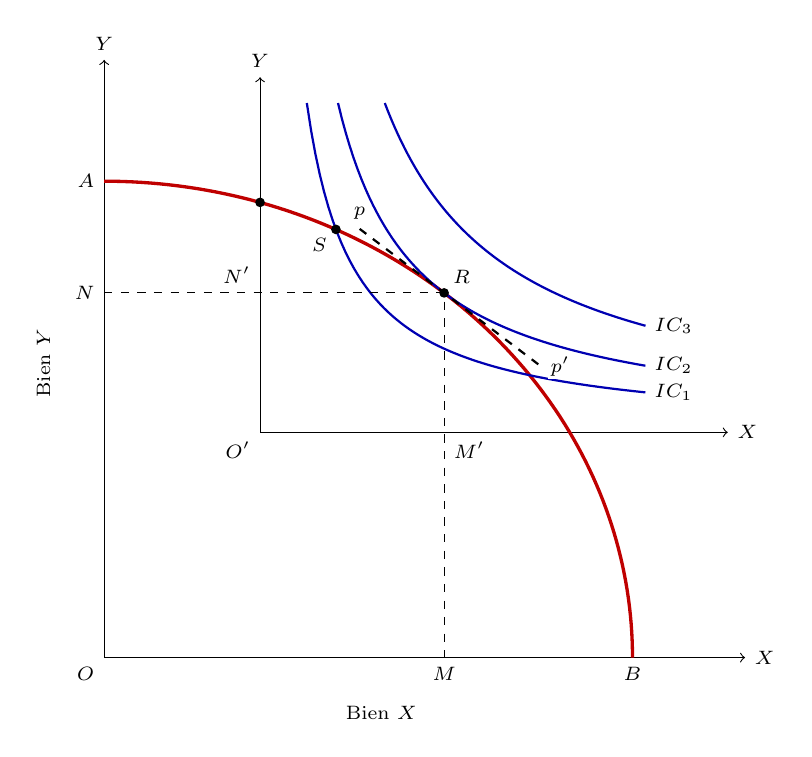
\begin{tikzpicture}[x=1.1cm,y=1.1cm,font=\scriptsize,
      dot/.style={circle,fill=black,inner sep=0pt,minimum size=3.5pt},
      ic/.style={blue!70!black,thick},
      lab/.style={fill=white,inner sep=0.8pt,outer sep=2.5pt,text=black}]
    % main axes
    \draw[->] (0,0) -- (7.4,0) node[right] {$X$};
    \draw[->] (0,0) -- (0,6.9) node[above] {$Y$};
    \node[below left] at (0,0) {$O$};
    \node[below] at (3.2,-0.45) {Bien $X$};
    \node[rotate=90] at (-0.7,3.4) {Bien $Y$};
    % inner axes
    \draw[->] (1.8,2.6) -- (7.2,2.6) node[right] {$X$};
    \draw[->] (1.8,2.6) -- (1.8,6.7) node[above] {$Y$};
    \node[below left] at (1.8,2.6) {$O'$};
    % the curve AB
    \draw[red!75!black,very thick] plot[domain=0:90,samples=90] ({6.1*cos(\x)},{5.5*sin(\x)});
    \node[left] at (0,5.5) {$A$};
    \node[below] at (6.1,0) {$B$};
    \node[dot] at (1.8,5.255) {};
    % courbes d'indifférence
    \draw[ic] plot[domain=2.34:6.25,samples=80] (\x,{2.6+2.053/(\x-1.8)}) node[right,lab] {$IC_1$};
    \draw[ic] plot[domain=2.70:6.25,samples=80] (\x,{2.6+3.422/(\x-1.8)}) node[right,lab] {$IC_2$};
    \draw[ic] plot[domain=3.24:6.25,samples=80] (\x,{2.6+5.475/(\x-1.8)}) node[right,lab] {$IC_3$};
    % R, its projections, and the common tangent
    \draw[dashed] (0,4.21) -- (3.925,4.21) -- (3.925,0);
    \draw[dashed,thick] (2.95,4.949) -- (5.05,3.357);
    \node[above,lab] at (2.95,4.949) {$p$};
    \node[right,lab] at (5.05,3.357) {$p'$};
    \node[dot] at (3.925,4.21) {};
    \node[above right,lab] at (3.925,4.21) {$R$};
    \node[dot] at (2.676,4.943) {};
    \node[below left,lab] at (2.676,4.943) {$S$};
    \node[left] at (0,4.21) {$N$};
    \node[above left] at (1.8,4.21) {$N'$};
    \node[below] at (3.925,0) {$M$};
    \node[below right] at (3.925,2.6) {$M'$};
  \end{tikzpicture}
  \captionof*{figure}{\small L'optimum du Product Mix. $AB$ is the frontière des possibilités
  de production. At $R$ the courbe d'indifférence $IC_2$ touches $AB$, with the
  common tangent $pp'$; $S$ is on $AB$ but on the lower $IC_1$. The dashed lines
  project $R$ on the main axes, at $N$ and $M$, and on the second pair of axes drawn
  from $O'$, at $N'$ and $M'$.}
\end{minipage}
\end{center}

\subsubsection{Les théorèmes du bien-être}

Two theorems link the efficacité de Pareto to the équilibre concurrentiel.

\begin{theorem}[Premier théorème du bien-être (\textit{first welfare theorem})]
  Tout équilibre concurrentiel est Pareto optimal.
\end{theorem}

Its reading is la \textbf{main invisible} (\textit{invisible hand}) d'Adam
Smith~: les acteurs maximisent leurs gains de manière individualiste et cela
résulte en une situation efficiente, celle qu'aurait choisie un \textbf{planificateur
social} (\textit{social planner}) qui maximise le surplus total. The surplus total
that planificateur maximises is the one the équilibre de marché was seen to maximise
above.

\begin{theorem}[Deuxième théorème du bien-être (\textit{second welfare theorem})]
  Toute allocation Pareto optimale peut être obtenue par un équilibre concurrentiel.
\end{theorem}

L'allocation peut être modifiée à l'aide d'\textbf{impôts forfaitaires}
(\textit{lump-sum taxes})~:
\begin{itemize}
  \item un impôt forfaitaire ne modifie pas les comportements~;
  \item dans la pratique, les impôts forfaitaires sont difficiles à mettre en
    œuvre~; politique de Thatcher à la fin des années 80.
\end{itemize}
The policy in question is the poll tax of the late 1980s in Britain, which met mass
protests calling for non-payment («~Pay no poll tax~»).

\subsubsection{Discussion}

The two theorems rest on assumptions:
\begin{itemize}
  \item ces théorèmes du bien-être supposent que tous les marchés sont à
    l'équilibre, en particulier le marché du travail~;
  \item pas de défaillances de marché~: monopoles, externalités, asymétries
    d'information, biens publics~;
  \item efficacité statique vs.\ dynamique.
\end{itemize}
The défaillances de marché are taken up in their own chapter; the contrast between
efficacité statique and efficacité dynamique is only named.

\subsubsection{Critiques du critère de Pareto}

Le \textbf{critère de Pareto} (\textit{Pareto criterion}) est l'objet de débats~:
\begin{itemize}
  \item pas de considérations de distribution des ressources (c'est une donnée du
    problème)~;
  \item pas de considération d'inégalités~;
  \item pas de notion de justice.
\end{itemize}

\subsubsection{Critiques d'Amartya Sen}

Amartya Sen's critiques are two.
\begin{itemize}
  \item Une économie avec des gens dans la misère et des gens très riches peut être
    Pareto optimale~: on ne peut pas améliorer la qualité de vie des plus pauvres
    sans réduire celle des plus riches.
  \item Le critère de Pareto confond utilité individuelle et bien-être qui ne
    dépend pas que de la consommation et du loisir et ignore~:
    \begin{itemize}
      \item les facteurs politiques et environnementaux~;
      \item les libertés individuelles et politiques~;
      \item le bien-être de la communauté.
    \end{itemize}
\end{itemize}

\subsection{L'approche de John Rawls}

Rawls starts from the worst-off: protéger les plus démunis = \textbf{critère
max-min} (\textit{maximin criterion}).\\

His device is the \textbf{voile de l'ignorance} (\textit{veil of ignorance})~: avant
que la société ne se forme, les gens ignorent leurs positions sociales, classes,
religions, génération. Behind the voile the question is «~quelles sont les règles à
adopter pour garantir une impartialité et une absence de biais~?~», and Rawls's
answer has two parts:
\begin{itemize}
  \item garantir les libertés individuelles de base~;
  \item \textbf{égalité des opportunités} (\textit{equality of opportunity}) et
    \textbf{principe de différence} (\textit{difference principle})~:
    \begin{itemize}
      \item tout le monde doit avoir une chance de réussir~;
      \item améliorer la position des plus démunis.
    \end{itemize}
\end{itemize}

\subsubsection{Critiques et influence}

The approach has its critics and a wide influence.
\begin{itemize}
  \item On taxe les plus riches, d'où problème d'incitations, en particulier
    l'innovation.
  \item Le lien avec l'efficience économique n'est pas démontré.
  \item Influence considérable en dehors de la philosophie politique et
    l'économie~: équité des algorithmes (robustes aux permutations).
\end{itemize}
Équité des algorithmes and robustness to permutations are only named.
